\chapter{Referencial Teórico}
\label{cap:referencial_teorico}
\section{Virtualização}
No contexto da computação, frequetemente uma alteração tecnológica torna alguma idéia obsoleta e ela desaparece rapidamente. Entretanto, outra mudança tecnológica poderia reavivá-la \cite{tanembaum}. Este é o caso da virtualização, dado que sua utilização teve oscilações ao longo do tempo. A principal motivação para virtualização nos começo dos anos 70 era aumentar o nivel de compartilhamento e utilização dos caros recursos computacionais tais como \textit{mainframes}\cite{menasce}. Nos anos 80 com a queda dos custos de hardware as grandes corporações trocaram os grandes e despediosos \textit{mainframes} por coleções de computadores pessoais, tendo assim a virtualização caído em desuso.

 Seu ressurgimento só viria acontecer, nos anos 90 dentro de um contexto ao qual tinha-se o crescimento de novos paradigmas computacionais, tais como cliente-servidor  e sistemas \textit{peer-to-peer}, aos quais suas estruturas eram constituídas basicamente de máquinas clientes conectadas à vários servidores. Esses novos ambientes trouxeram com eles diversos desafios e problemas incluindo confiabilidade, segurança, aumento no custo de administração e complexidade, espaço fisico e consumo de energia \cite{menasce}. Desse modo, o ressurgimento da virtualização vem promovendo a mitigação de tais problemas recorrentes nesses novos paradigmas computacionais ( alteração tecnológica).
 
\subsection{Conceituação} 
Pode se definir que Virtualização é a técnica que permite particionar um único sistema computacional em vários outros denominados de máquinas virtuais. Cada máquina virtual oferece um ambiente completo muito similar a uma máquina física. Com isso, cada máquina virtual pode ter seu próprio sistema operacional, aplicativos e serviços de rede (Internet) \cite{carissimi}. A virtualização pode ser feita das seguintes formas:

\begin{itemize}
\item \textbf{Virtualização de servidores:} a mais comum e fácil de ser justificada. Diferente da época dos \textit{mainframes}, a virtualização agora é feita em servidores \textit{x86}.

\item \textbf{Virtualização de \textit{desktops}:} trata da configuração dos \textit{desktops} dos usuários finais em uma infraestrutura centalizada virtual. Isso signfica que as aplicações de desktop também passam a executar em um \textit{datacenter}, sob a forma de máquinas virtuais. Esse é o conceito de \textit{Virtual Desktop Infrastructure(VDI)}, que permite a montagem dinâmica de \textit{desktops}, oferecendo maior confiabilidade e otimização do uso de espaço em disco com a consollidação do armazenamento e flexibilidade na escolha do sistema peracional \cite{manoel}.

\item \textbf{Virtualização do armazenamento(\textit{storage})}: a ideia é introduzir um componente que permite às diversas unidade heterogêneas de armazenamento(discos físicos) serem vistas como um conjunto homogêneo de recursos \cite{manoel}.

\item \textbf{Virtualização das aplicações:} trata do conceito de execução do programa por completo, em um repositório central, permitindo a configuração centralizada do aplicativo, o que melhora seu gerenciamento, por permitir que seja feita em um único lugar \cite{manoel}. 

\item \textbf{Virtualização de redes: } Arquitetura que proporciona um ambiente de rede separado para cada grupo ou organização. Esses ambientes lógicos são criados sobre uma única infraestrutura compartilhada de rede \cite{manoel}.

\end{itemize}

Uma outra abordagem que pode ser utilizada para conceituar a virtualização é defini-la como uma camada de abstração entre o hardware e o software, que protege o acesso direto do software aos recursos físicos do hardware. A forma pela qual essa camada de abstração é implementada dá origem às máquinas virtuais de processo e aos monitores de máquinas virtuais também chamados de \textit{hypervisor} \cite{manoel}.

\begin{figure}[!htb]
\centering
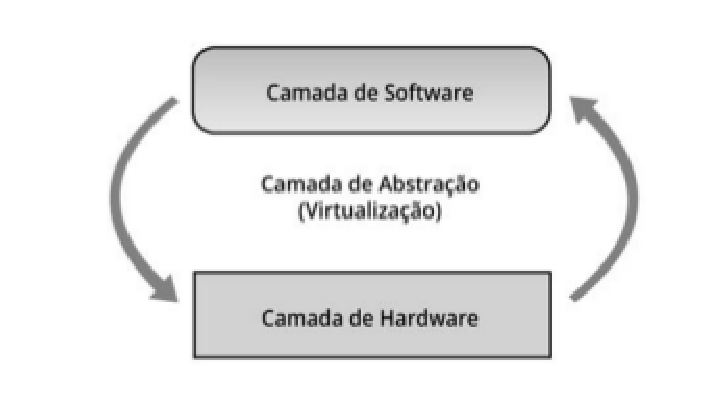
\includegraphics [keepaspectratio=true,scale=0.60]{figuras/virtualization_role.eps}
\caption{Responsabilidade da virtualização}
\cite{manoel}.
\label{virtualization_role}
\end{figure}

\subsection{Máquinas virtuais}
Uma máquina virtual é uma abstração em software de uma máquina física real. Destaca-se que é executada como uma aplicação padrão de usuário sobre um sistema operacional. A própria máquina virtual emula uma máquina física possuindo assim seus próprios discos e dispositivos \cite{mcewan}. Desse modo, umas das vantagens de máquinas virtuais reside na independência de uso do seu sistema operacional com relação ao sistema operacional da máquina física ao qual se encontra. Assim, em uma máquina física pode-se executar várias máquinas virtuais cada uma delas com sistemas operacionais diversos. A imagem \ref{arc_virtualization}, apresenta a arquitetura de um ambiente virtualizado dividido em duas camadas: \textit{software} e \textit{hardware}. É na camada de software, mais espceficamente na camada de virtualização, através dos \textit{hypervisor}, que são providos as máquinas virtuais (hóspedes) com seus respectivos sistemais operacionais e \textit{hardwares} virtuais.  

\begin{figure}[!htb]
\centering
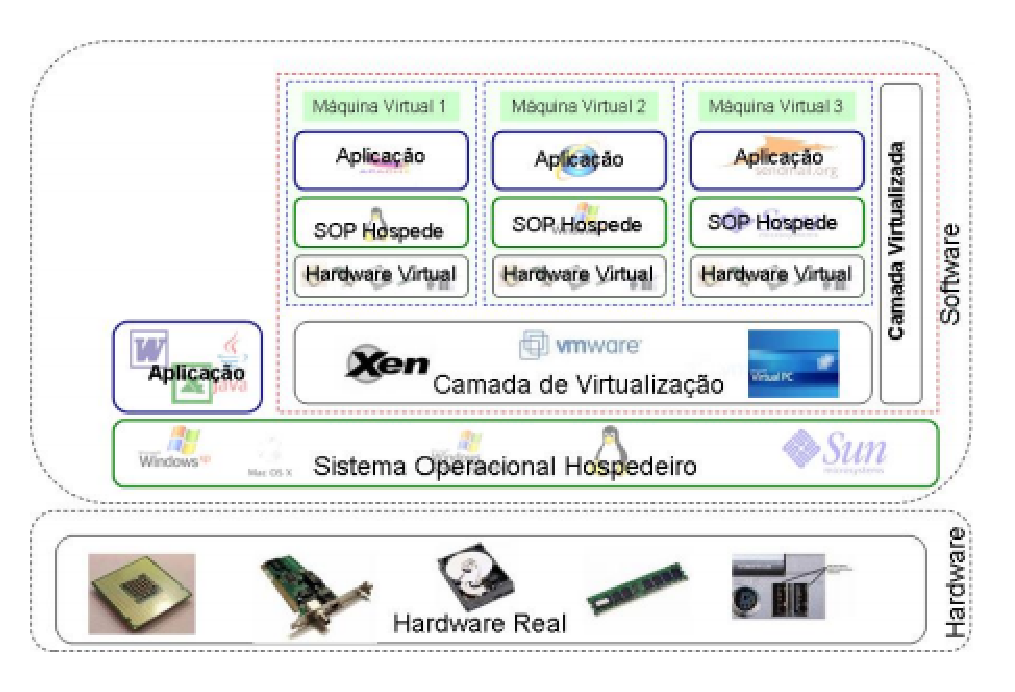
\includegraphics [keepaspectratio=true,scale=0.40]{figuras/virtualization_arc.eps}
\caption{Representação da implementação de um ambiente virtual}
\cite{junior}.
\label{arc_virtualization}
\end{figure} 
 
\subsection{Monitor de Máquinas virtuais}
O \textit{hypervisor} (ou também conhecido como monitor de máquinas virtuais) é o software que possui mecanismos capazes de prover máquinas virtuais. Suas principais funções consistem no esclanomaneto de tarefas, gerência da memória e manutenção do estado da máquina virtual \cite{manoel}. Desse modo, atributos como desempenho e escalabilidade são determinantes para definir a qualidade dos serviços fornecidos por um \textit{hypervisor}. Algumas características são essenciais a um \textit{hypervisor}: segurança sobre os recursos virtualizados e agilidade na reconfiguração de recursos computacionais, sem interromper as operações do servidor de máquinas virtuais \cite{manoel}. Os \textit{hypervisors} são classificados em dois tipos:

\begin{itemize}
\item \textbf{Tipo I}(\textit{bare metal}, nativo ou supervisor):executa diretamente no hardware do servidor. Controla o hardware e o acesso do sistema operacional convidado(\textit{guest OS}. O papel do \textit{hypervisor} nativo é compartilhar os recursos de hardware entre as máquinas virtuais, de forma que cada uma delas imagina ter recursos exclusivos \cite{manoel}. Exemplos desse tipo incluem: \textit{Oracle Virtual Box}, \textit{VMware workstation}.

\item \textbf{Tipo II}(hosted): aplicação que fornece um ambiente de execução para outras aplicações. Executa sob um sistema operacional nativo como se fosse um processo deste. A camada de virtualização é composta por um sistema operacional hóspede e um hardware virtual, que são criados sobre os recursos de hardware oferecidos por meio do sistema operacional nativo \cite{manoel}. Exemplos desse tipo incluem: \textit{Oracle Virtual Box}, \textit{VMware workstation}.
\end{itemize}

\subsection{Tipos de virtualização}
A virtualização pode ser realizada de diferentes maneiras, cada uma com seus prós e contras. Na prática, em arquiteturas x86, as opções de virtualização alteram o nível de privilégios (\textit{rings}) padrões. As soluções baseadas em \textit{hypervisor} inclui a virtualização completa e a paravirtualização \cite{manoel}. Exemplos desse tipo incluem: \textit{KVM}, \textit{ Hyper-V}, \textit{XEN}

Na virtualização total, uma estrutura completa de hardware é virtualizada, portanto o sistema a ser virtualizado (sistema convidado) não precisa sofrer qualquer tipo de alteração. O principal benefícios da virtualização total é justamente o fato de que o sistema a ser virtualizado não sofre qualquer tipo de alteração \cite{marcos}. Entretanto, o sistema virtualizado executa de forma mais lenta e o monitor de máquinas virtuais precisa implementar alternativas para que as operações privilegidas possam ser executadas em procesadores que não suportem a virtualização nativamente \cite{marcos}.

\begin{figure}[!htb]
\centering
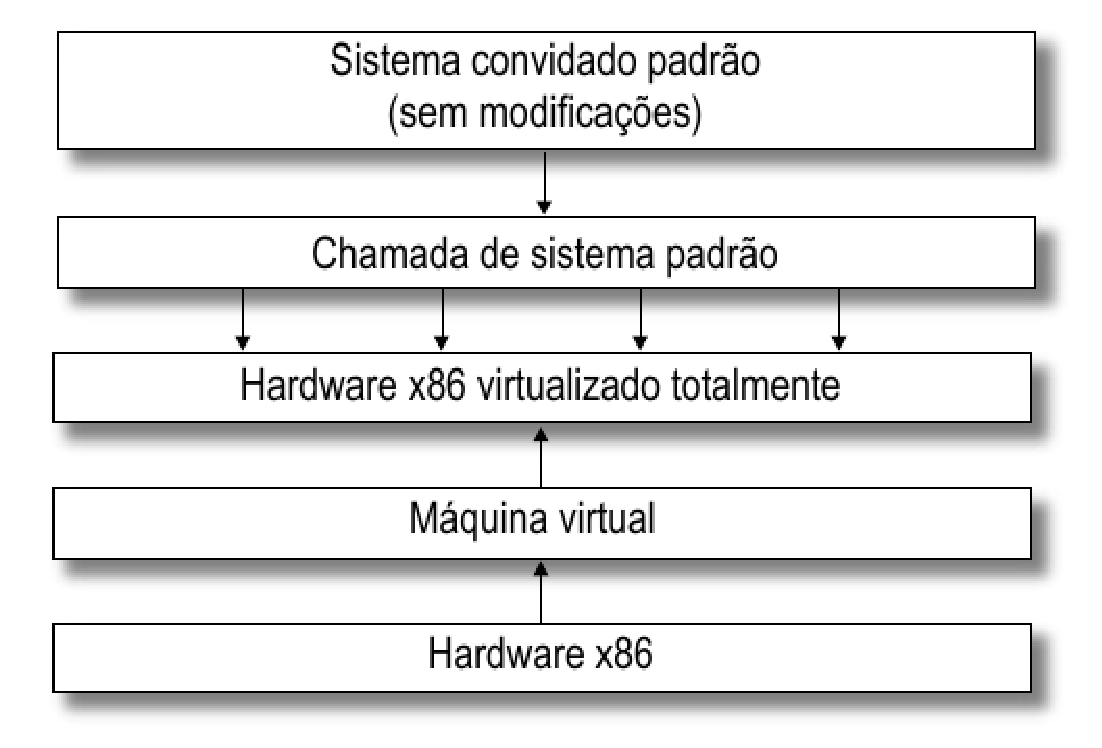
\includegraphics [keepaspectratio=true,scale=0.30]{figuras/full_virtualization.eps}
\caption{Representação da virtualização total}
\cite{marcos}.
\label{full_virtualization}
\end{figure}

Na paravirtualização, o sistema a ser virtualizado (sistema convidado) sofre modificações para que a interação com o monitor de máquinas virtuais seja mais eficiente. A paravirtualização permite que o sistema convidado consiga acesar recursos do hardware diretamente. O acesso é monitorado pelo monitor e máquinas virtuais, que fornece ao sistema convidado todos os "limites" do sistema, tais como endereços de memória que podem ser utilizados e endereçamento em disco, por exemplo \cite{marcos}.

\begin{figure}[!htb]
\centering
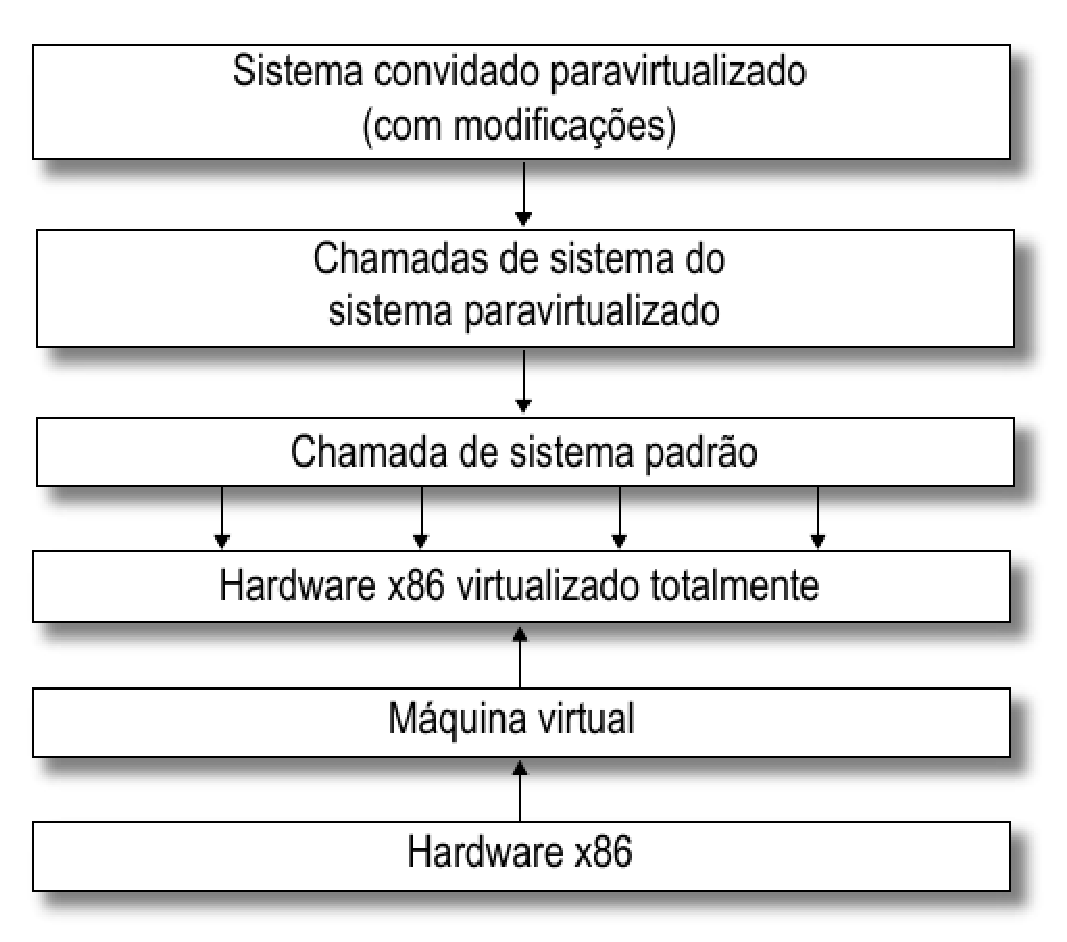
\includegraphics [keepaspectratio=true,scale=0.3]{figuras/paravirtualization.eps}
\caption{Representação da virtualização total}
\cite{marcos}.
\label{paravirtualization}
\end{figure}

\subsection{Ferramentas de Virtualização}
Nessa seção serão abordadas algumas das ferramentas principais utilizadas para provimento de ambientes virtualizados: \textit{Xen, KVM}. As ferramentas de virualização basicamente são as plataformas responsáveis por prover a camada de virtualização responsável pela disponibilização de máquinas virtuais.

O KVM é uma solução de virtualização total voltada para arquiteturas x86, possui suporte para tecnologias de virtualização \textit{Intel VT} e \textit{AMD-V}. Foi incorporado ao kernel em janeiro de 2007, tornando-se assim um componente do linux sendo capaz de herdar as funcionalidade principais do mesmo \cite{redhatkvm,qumranet}.Pelo fato do KVM ter sido incorporado ao kernel do linux, o seu desenvolvimento passou a ter a colaboração ativa e o suporte da ampla comunidade do linux bem como de algumas fornecedoras da industria do software tais como, Red Hat, AMD, HP, IBM, Intel, Novell, Siemens, SGI entre outros\cite {redhatkvm}.

A arquitetura do KVM é implementada como um processo convencional do linux, de modo que cada CPU virtual aparece como um processo regular. Proporcionando assim, ao KVM os beneficios de todas as funcionalidades do kernel do linux\cite{redhatkvm}. A emulação dos dispositivos e as operações de entrada e saída nos sistemas operacionais hóspedes, fica por conta de uma versão modificado do QEMU \cite{redhatkvm,qumranet}. Neste, caso o KVM intercepta eventos a niveis de sistema que precisam ser emulados, tais como leitura do disco ou o envio de um pacote pela rede, e invoca o QEMU que emula a funcionalidade do \textit{hardware} requsitado \cite{rasmusson}. Por exemplo, a placa de rede virtual da máquina virtual que precisasse ser usada para algum envio de pacotes pela rede, teria esse tipo de funcionalidade emulada a partir da placa de rede física da máquina hospedeira. 

\begin{figure}[!htb]
\centering
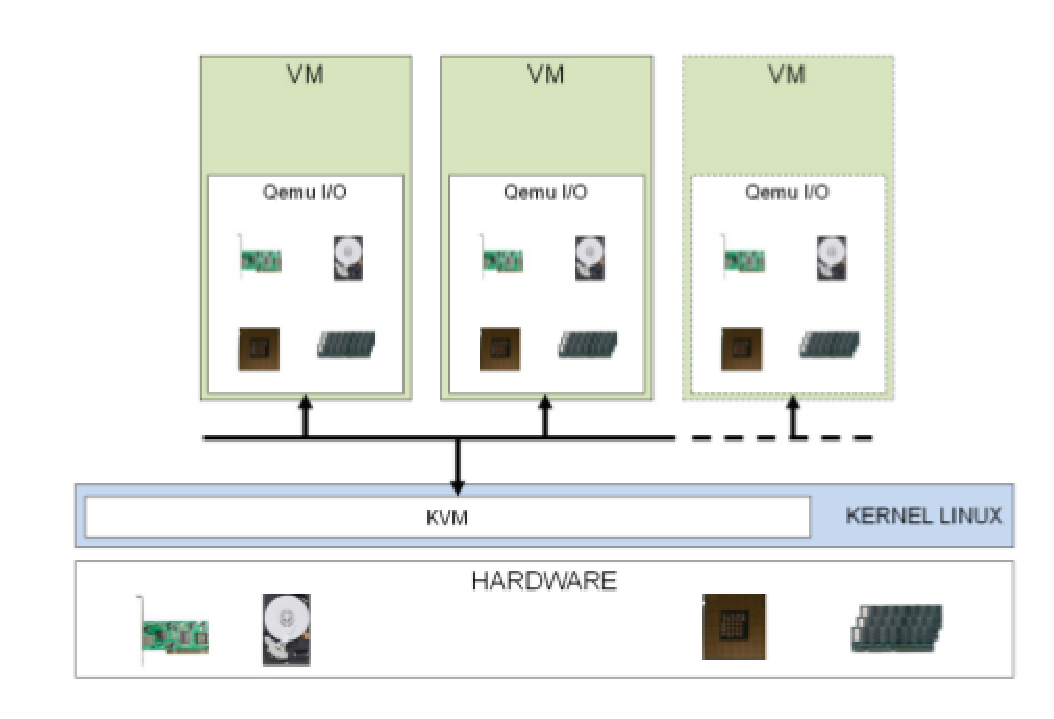
\includegraphics [keepaspectratio=true,scale=0.6]{figuras/kvm_arc.eps}
\caption{Arquitetura do KVM}
\cite{fabiano}.
\label{kvm_arc}
\end{figure}

Já o XEN foi criado por Keir Fraser e Ian pratt como parte do projeto de pesquisa \textit{Xenoserver} pela \textit{Cambridge University}. Sendo que em 2002, teve seu código fonte aberto afim de promover melhorias no mesmo com a contribuição da comunidade de desenvolvedores. É um dos mais populares \textit{hypervisor} a implementar técnica de paravirtualização\cite{xen}. Desse modo é conhecido por possuir uma baixa perda de desempeho, se aproximando da performance nativa do servidor\cite{walters}.Isso é justificado pelo fato de que o sistema operacional das máquinas virtuais é modificado de modo que as chamadas privilegiadas são substituidas por chamadas diretas ao \textit{hypervisor}, ao contrário do que é feito com abordagens que utilizam emulação e tradução binária que acabam por focar no gerenciamento de chamadas previlegiadas \cite{redhatkvm}. 

A arquitetura do XEN é composta por dois dois componentes: o próprio \textit{hypervisor} XEN e pelo domínio 0 (ou Dom0). O \textit{hypervisor} XEN é responsável por virtualização de memória e CPU, gerenciamento de energia e escalonamento das máquinas virtuais. Enquanto que o Dom0 é uma máquina virtual instanciada pelo próprio \textit{hypervisor} XEN que possui acesso direto ao hardware, sendo responsável por prover \textit{drivers} dos dispostivos de E/S para máquinas virtuais \cite{redhatkvm}. As máquinas virtuais são conhecidas como DomU(\textit{unprivileged domain}), sendo que as operações feitas por dispositivos de E/S são realizadas através da comunicação entre o processo \textit{front end}, existente no núcleo modificado das DomU, e o processo \textit{back end}, existente no núcleo da Dom0 \cite{redhatkvm}.

\begin{figure}[!htb]
\centering
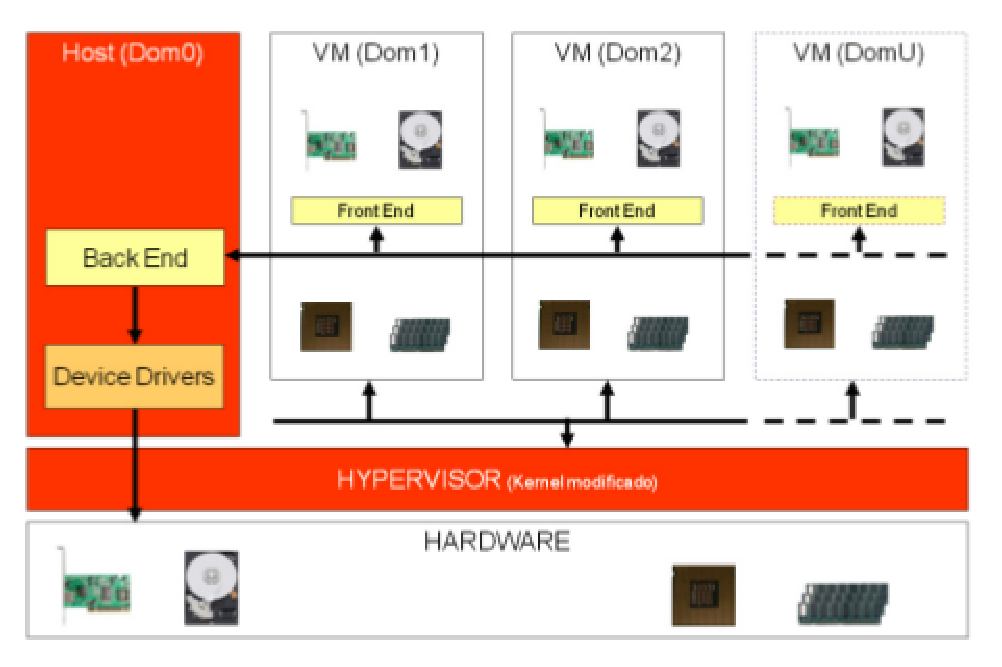
\includegraphics [keepaspectratio=true,scale=0.65]{figuras/xen_arquitecture.eps}
\caption{Arquitetura do KVM}
\cite{fabiano}.
\label{xen_arquitecture}
\end{figure}

\section{Trabalhos relacionados}
Esse seção tem como intuito expor alguns trabalhos relacionados à análise de desempenho. Esses trabalhos também servirão de insumo para desenvolvimento do estudo de interferência de desempenho proposto por este trabalho.

No trabalho apresentado por \cite{koh2007} é feito um estudo de interferência entre aplicações executadas sobre o mesmo \textit{hardware} a partir de máquinas virtuais. Como cargas de trabalho, foram escolhidas aplicações do mundo real utilizadas para compressão, compilação de código fonte, e renderização de \textit{frames}, bem como fora utilizadas ferramentas voltadas para testes de desempenho (\textit{benchmark}). Essas ferramentas foram escolhidas visando o teste de vários aspectos do sistema e \textit{hardware}.

\begin{table}[!h]
\centering
%\cite{koh2007}
\caption{Aplicações utilizadas para testes de desempenho \cite{koh2007}.}
\label{applications}
\resizebox{0.6\textwidth}{!}{
\begin{tabular}{|l|c|lll}
\cline{1-2}
Name        & \multicolumn{1}{l|}{Maior recurso utilizado} &  &  &  \\ \cline{1-2}
Add\_double & CPU                                          &  &  &  \\ \cline{1-2}
Analyser    & Memória                                      &  &  &  \\ \cline{1-2}
Bw\_mem     & Memória                                      &  &  &  \\ \cline{1-2}
Bzip2       & Misto                                        &  &  &  \\ \cline{1-2}
Cat         & Disco                                        &  &  &  \\ \cline{1-2}
Cachebench  & Memória                                      &  &  &  \\ \cline{1-2}
Cachebuster & Memória                                      &  &  &  \\ \cline{1-2}
Ccrypt      & Misto                                        &  &  &  \\ \cline{1-2}
Cp          & Disco                                        &  &  &  \\ \cline{1-2}
Dd          & Disco                                        &  &  &  \\ \cline{1-2}
Grep        & Disco                                        &  &  &  \\ \cline{1-2}
Gzip        & Misto                                        &  &  &  \\ \cline{1-2}
Iozone      & Disco                                        &  &  &  \\ \cline{1-2}
Make        & Misto                                        &  &  &  \\ \cline{1-2}
Povray      & Misto                                        &  &  &  \\ \cline{1-2}
Spinlock    & CPU                                          &  &  &  \\ \cline{1-2}
\end{tabular}}
\end{table}

Para cálculo da interferencia é feita a seguinte abordagem: Duas máquinas virtuais são criadas (denomina-se "domínio 1" e "domínio 2") em um servidor executando o \textit{hypervisor XEN},  uma aplicação F é executada no domínio 1 contra domínio 2 sem qualquer aplicação sendo executada, o desempenho da aplicação F neste cenário é medido. Em seguida, essa mesma aplicação F é executada contra uma aplicação B que está sendo executada em domínio 2, o desempenho de F e medido novamente. O calculo da interferência de uma aplicação F contra B é feito dividindo o desempenho de F executado contra aplicação B, pelo desempenho do próprio F contra o domínio sem qualquer aplicação. Tal procedimento é feito para os seguinte conjunto de métricas: Média de uso de CPU, \textit{cache hits}, \textit{cache misses}, troca de máquinas virtuais por segundo, bloqueio de operações de entrada e saída por segundo, tempo de emissão de leitura e escrita por segundo e tempo gasto na leitra e escrita por máquina virtual. 

De maneira geral, a observação feita neste trabalho é que determinadas aplicações podem sofrer mais interferências de outras aplicações que possuem o mesmo uso de tipo de recurso. O exemplo disso é apresentado Figura \ref{interference_app}, onde uma aplicação executada sem interferência alcança uma pontuação de 1. Duas aplicações que não interferem uma com a outra alcança uma pontuação perto de 2, como grep+povray. Já executando grep+grep a pontuação cai para 0.35 %Por exemplo, uma aplicação A que costuma consumir mais CPU, pode sofrer mais interferência de uma outra aplicação que possui a mesma característica, do que de uma aplicação que realiza operações mais focadas na escrita de disco. Além disso, é proposto por esse trabalho que com resultados desses desempenhos pode se fazer predição de desempenho de uma aplicação qualquer, a partir de analise matemáticas.

\begin{figure}[!htb]
\centering
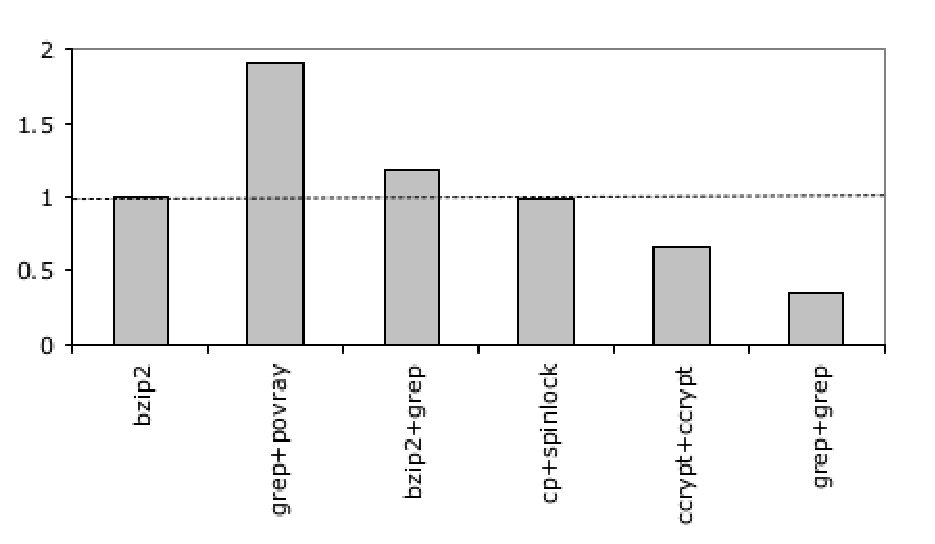
\includegraphics [keepaspectratio=true,scale=0.65]{figuras/interference_aplications.eps}
\caption{Variação de desempenho para combinações diferentes de aplicações}
\cite{koh2007}.
\label{interference_app}
\end{figure}

Além disso, é proposto por esse trabalho que com resultados desses desempenhos pode se fazer predição de desempenho de uma aplicação qualquer, a partir de análises matemáticas. Dado a quantidade variáveis, que são as métricas utilizadas para medição de desempenho, as análises matemáticas escolhidas foram a análise de componente principal e a análise de regressão linear. Um comparativo entre as análises foi feito de modo que chegou-se a conclusão que análise por PCA apresentava uma porcentagem de erro menor. Esse trabalho demonstrou que a taxa de erro utilizando o modelo PCA se manteve igual, mesmo utilizando outros servidores físicos com configurações diferentes. Entretanto, uma das restrições deste trabalhos é que o mesmo fora aplicado em aplicações que estavam sendo executadas em duas máquinas virtuais. Desse modo como trabalhos futuros é proposta a investigação no uso de mais máquinas virtuais, e aplicação de modelos não lineares para predição de desempenho bem como a adição de novos tipos de métricas que envolvam outras características a nivel de sistema, tal como desempenho de aplicações de rede.

No trabalho de \citeonline{popiolek2012}, disserta sobre a importância de se utilizar métricas nativas (Tabela \ref{metric_tools}) de sistemas  operacionais tais como \textit{Linux} e \textit{Windows} para detecção de gargálos de performance. Esse trabalho acaba focando na aferição de operações de entrada e saída memória e uso de CPU, utilizando ferramentas de bencharmking para geração de cargas de trabalho. Seus cenários de teste são basicamente variando de uma a seis máquinas virtuais, sendo que o hypervisor utilizado é o KVM. As análises permitem mostrar a queda de desempenho como um todo quando se tem o aumento do número de máquinas virtuais em em execução (Imagem \ref{iobound_experiments}). Como trabalho futuros, proponhe-se que sejam análise estatísticas afim de comprovar possíveis relações entre as métricas observadas, alem de determinar o limiar que um sistema pode operar sem ter perda significativa no desempenho.

% Please add the following required packages to your document preamble:
% \usepackage{multirow}
\begin{table}[]
\centering
\caption{Contadores de desempenho de disco para \textit{Windows} e \textit{Linux} \cite{popiolek2012}}
\label{metric_tools}
\resizebox{1.0\textwidth}{!}{
\begin{tabular}{lllll}
\cline{1-4}
\multicolumn{1}{|l|}{Windows}                & \multicolumn{2}{l|}{Linux}                                             & \multicolumn{1}{c|}{\multirow{2}{*}{Descricao}}                                                                                                  &  \\ \cline{1-3}
\multicolumn{1}{|l|}{Monitor de Desempenho}  & \multicolumn{1}{l|}{iostat}          & \multicolumn{1}{l|}{df}         & \multicolumn{1}{c|}{}                                                                                                                            &  \\ \cline{1-4}
\multicolumn{1}{|l|}{\%Idle Time}            & \multicolumn{1}{l|}{-}               & \multicolumn{1}{c|}{-}          & \multicolumn{1}{c|}{\begin{tabular}[c]{@{}c@{}}Porcentagem de tempo\\  que o disco permanece inativo\end{tabular}}                               &  \\ \cline{1-4}
\multicolumn{1}{|l|}{(Disk Bytes/sec)/ 1024} & \multicolumn{1}{l|}{(rKB/s)+(wKB/s)} & \multicolumn{1}{c|}{-}          & \multicolumn{1}{c|}{\begin{tabular}[c]{@{}c@{}}Número de Kilobytes \\ lidos/escritos por segundo\end{tabular}}                                   &  \\ \cline{1-4}
\multicolumn{1}{|l|}{Disk Transfers/sec}     & \multicolumn{1}{l|}{(r/s)+(w/s)}     & \multicolumn{1}{c|}{-}          & \multicolumn{1}{c|}{\begin{tabular}[c]{@{}c@{}}Número de requisições\\  por segundo completadas\end{tabular}}                                    &  \\ \cline{1-4}
\multicolumn{1}{|l|}{Split IO/sec}           & \multicolumn{1}{c|}{-}               & \multicolumn{1}{c|}{-}          & \multicolumn{1}{c|}{\begin{tabular}[c]{@{}c@{}}Número de requisições por segundo\\  que foram divididas\\ em múltiplas requisições\end{tabular}} &  \\ \cline{1-4}
\multicolumn{1}{|l|}{Free Megabytes}         & \multicolumn{1}{c|}{-}               & \multicolumn{1}{l|}{Disponível} & \multicolumn{1}{c|}{\begin{tabular}[c]{@{}c@{}}Megabytes disponíveis para uso\\  em unidade de armazenamento\end{tabular}}                       &  \\ \cline{1-4}
\multicolumn{1}{|l|}{Avg. Disk sec/Transfer} & \multicolumn{1}{l|}{Await}           & \multicolumn{1}{c|}{-}          & \multicolumn{1}{l|}{Média de tempo para completar uma requisição}                                                                                &  \\ \cline{1-4}
\multicolumn{1}{|l|}{Avg. DIsk Queue Length} & \multicolumn{1}{l|}{avgqu-sz}        & \multicolumn{1}{c|}{-}          & \multicolumn{1}{c|}{\begin{tabular}[c]{@{}c@{}}Média de tamanho de filas de requisições\\  esperando pelo disco rígido\end{tabular}}             &  \\ \cline{1-4}
                                             &                                      &                                 &                                                                                                                                                  &  \\
                                             &                                      &                                 &                                                                                                                                                  &  \\
                                             &                                      &                                 &                                                                                                                                                  &  \\
                                             &                                      &                                 &                                                                                                                                                  &  \\
                                             &                                      &                                 &                                                                                                                                                  &  \\
                                             &                                      &                                 &                                                                                                                                                  &  \\
                                             &                                      &                                 &                                                                                                                                                  &  \\
                                             &                                      &                                 &                                                                                                                                                  & 
\end{tabular}}
\end{table}

\begin{figure}[!htb]
\centering
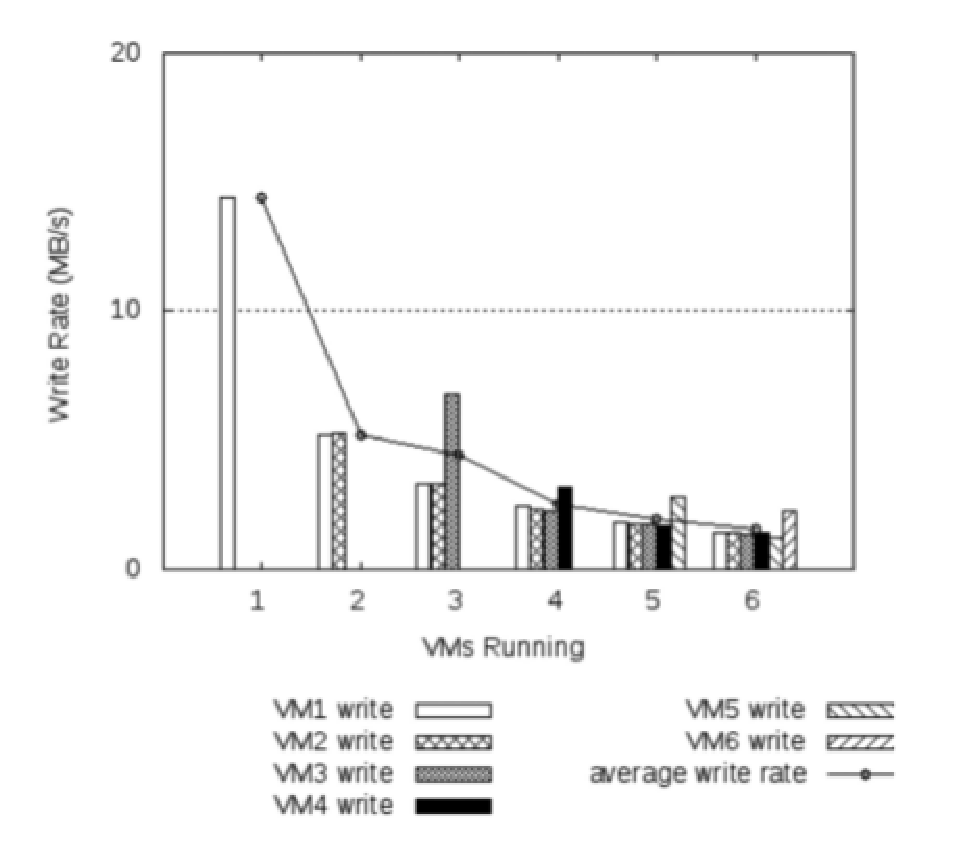
\includegraphics [keepaspectratio=true,scale=0.65]{figuras/iobound_experiments.eps}
\caption{Taxa de escrita em disco para experimentos voltados para E/S.}
\cite{popiolek2012}.
\label{iobound_experiments}
\end{figure}

Por fim, o trabalho de \citeonline{huber2011} tem como intuito prover um modelo genérico de predição de desempenho a partir de determinados fatores que podem interferir na virtualização. A idéia é que esse modelo genérico seja aplicável em diferentes tipos plataformas de virtualização. Assim, neste trabalho os experimentos são aplicados nos \textit{hypervisors } \textit{Citrix XenServer 5.5} e \textit{VMware ESX 4.0}. Os fatores categorizados para os experimentos foram: tipo de virtualização, configuração de gerenciamento de recursos e perfis de cargas de trabalho. Para o tipo de virtualização, os experimentos consistem em observar a perda de desempenha ocasionada com a virtualização. Na categoria de configuração de gerenciamento de recursos, são considerados fatores de configuração como número de máquinas virtuais e afinidade de núcleo. E para cargas de trabalho, foram executadas algumas ferraments de \textit{benchmarking} a fim de se analisar diversas cargas de trabalho. Para o modelo de predição, fora utlizada análise de regressão linear assim como feito em \citeonline{koh2007}.

\begin{figure}[!htb]
\centering
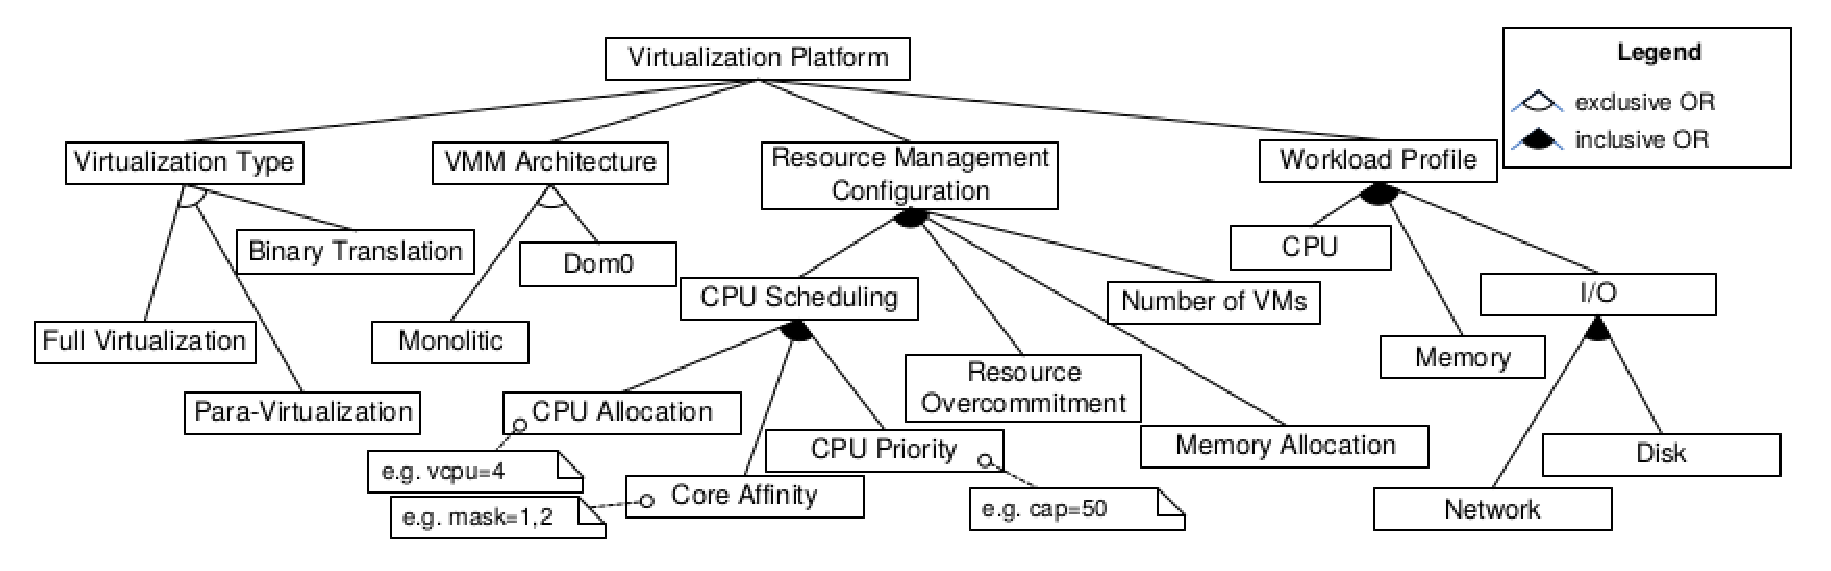
\includegraphics [keepaspectratio=true,scale=0.50]{figuras/factors_influence.eps}
\caption{Fatores que influenciam no desempenho de plataformas virtualizadas}
\cite{huber2011}.
\label{influence_factors}
\end{figure} 
%Xen é um hipervisor do tipo 1 (ou baremetal) \textit{open source} para arquiteruas x86 que utiliza, por padrão a técnica de paravirtualização, \cite{clark}. Uma das maiores vantagens do uso do Xen como VMM na para-virtualização é o fato de que este apresenta um desempenho melhor do que os produtos de virtualização total, quando a máquina física hospedeira não tem instruções de hardware de suporte a virtualização \cite{eder}  

